\section{Relation to individual-state geometry}\label{sec:geometry}
Manuscript~I~\cite{PaperI} attached to a single state a geometry; here only the integer part is needed. Two facts about it are taken from the programme's releases and are \stat{cited}, not re-proved.
\begin{itemize}[leftmargin=1.6em,itemsep=1pt]
\item \emph{Collapse of integer state geometry (B2-T1).} For an integer $x$ put $\sigma(x)=\prod_pp^{\lfloor v_p(x)/2\rfloor}$. The complete geometric record of $x$ is a function of $\sigma(x)$ alone, equivalent to the occurrence set $D(x)$ (the divisors $\ge2$ of $\sigma(x)$); all its topological invariants are trivial and the move complex $\Kmove(x)$ of an integer state is contractible. What varies between integers is dimension, shape, the $f$-vector and the inclusion order.
\item \emph{Different objects.} $\Kmove(x)$ lives on the occurrence set of one state; the history complexes of this manuscript live on admissible words from a fixed source. They are not identified.
\end{itemize}
\begin{proposition}[obstruction to detecting histories by state homology]\label{prop:A4T7}
Every integer endpoint $E$ of a SELECT-II history has $\Kmove(E)$ contractible (cited). Hence no homological invariant of $\Kmove(E)$ can detect the component structure of the histories ending at $E$. Witnesses: the endpoints $9000$, $48000$, $392000$ have $2$, $3$, $3$ components of histories with contents $\{2,4\}\cup A$, $A=\{5,9\},\{5,9,3\},\{5,9,3,6\}$ (source $4$; recomputed in this work, \cref{ex:R3T3}), and the order bit $I=[2\text{ before }4]$ is constant on components and takes both values (\cref{thm:R3T3}); each $\Kmove(E)$ has $\mathbb F_2$-Betti vector $(1,0,0,0)$ (cited). \stat{cited} for the contractibility; \stat{finite-exact} for the component counts.
\end{proposition}
\provx{A4-T7}{GEO\_HD\_BRIDGE\_v004:A4-T7 (obstruction)}{cited}{cited}
\begin{figure}[tbp]\centering
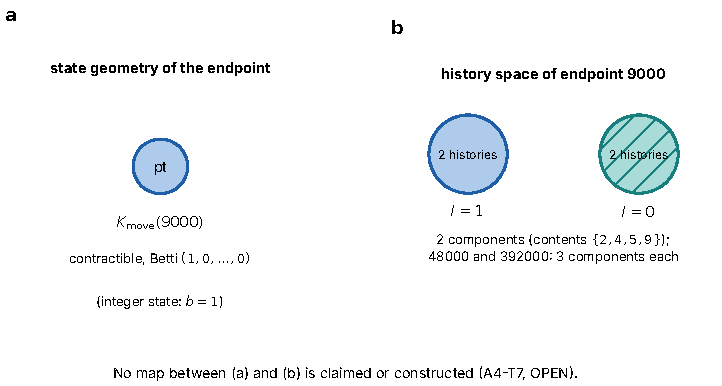
\includegraphics[width=\linewidth]{fig20_state_vs_history}
\caption{\textbf{Contractible state geometry against a disconnected history space (schematic, data finite-exact).} (a) The state geometry of the endpoint $9000$ is a point up to homotopy: $\Kmove(9000)$ is contractible with Betti vector $(1,0,0,0)$ (cited). (b) The swap-class structure of the histories of $\{2,4,5,9\}$ from source $4$ ending at $9000$: two components of two histories each, distinguished by $I$ (exact). The picture is schematic; no map between (a) and (b) is claimed or constructed. Theorem illustrated: \cref{prop:A4T7}.}\label{fig:state}
\end{figure}
\noindent The figure above is \cref{fig:state}; its caption states the exactness of what is drawn.
What is \emph{not} established. No functor, map or inequality between $H_*(\Kmove)$ and the homology of a history complex is claimed. A direct comparison would need an invariant of rational states that is meaningful for histories without extending SELECT-II, which the model boundary of this manuscript excludes; the question whether such an invariant exists is open (\cref{sec:synthesis}). The only integer-level connection proved here is the occurrence-event one: the fibre sequence of a history is built from $D(x_i)=D(\sigma(x_i))$ (\cref{thm:faith}), so the state geometry of the visited states determines the fibre sequence while the state geometry of the endpoint alone does not (\cref{prop:A4T7}).
